\documentclass{article}

% Submission mode (anonymized). Switch to [final] for camera-ready with author info,
% or [preprint] for a named arXiv-style version.
\PassOptionsToPackage{numbers, compress}{natbib}
\usepackage{neurips_2024}

\usepackage[utf8]{inputenc}
\usepackage[T1]{fontenc}
\usepackage{hyperref}
\usepackage{url}
\usepackage{booktabs}
\usepackage{amsfonts}
\usepackage{amsmath}
\usepackage{nicefrac}
\usepackage{microtype}
\usepackage{xcolor}
\usepackage{graphicx}
\usepackage{caption}
\usepackage{subcaption}
\usepackage{multirow}
\usepackage{enumitem}

\title{Where Does the Gain Come From? Attributing Spatio-Temporal\\Forecasting Improvements on METR-LA}

\author{%
  Anonymous Author(s) \\
  Affiliation \\
  Address \\
  \texttt{email}
}

\begin{document}
\maketitle

\begin{abstract}
Spatio-temporal graph neural networks (ST-GNNs) routinely outperform temporal-only baselines on traffic forecasting benchmarks, but the literature rarely quantifies \emph{which} component of the architecture delivers the gain. We perform a controlled, one-factor-at-a-time decomposition on METR-LA across sixteen iterations, with multi-seed validation of the headline configurations. The temporal-only LSTM baseline achieves test RMSE $15.00$ mph. Our best spatio-temporal model reaches $11.92 \pm 0.02$ (3-seed) --- a $20.5\%$ relative reduction. Decomposing this gain reveals that $94\%$ comes from a single architectural fix --- treating each sensor as an independent time series before message passing --- while only $\approx 5\%$ comes from the graph layer itself; sub-$0.05$ RMSE refinements (training length, layer depth, attention vs.\ spectral operators) lie at or below the seed-noise floor of $0.019$ RMSE and cannot be claimed as real effects. Among graph-side levers, only topology (correlation vs.\ physical adjacency) produces a measurable effect; operator choice (GAT vs.\ ChebConv) is null. The contribution is methodological: a multi-seed attribution table that recovers a much smaller defensible spatial contribution than the headline RMSE suggests.
\end{abstract}

\section{Introduction}
\label{sec:intro}

Traffic forecasting on sensor networks such as METR-LA \cite{li2018dcrnn} is a canonical spatio-temporal task: a $\sim 1$~hour history of speed measurements across $207$ Los Angeles freeway sensors is used to predict speeds over the following hour. Spatio-temporal graph neural networks --- combining a recurrent or convolutional temporal encoder with a graph-convolutional spatial operator over a sensor adjacency --- have driven a decade of headline-RMSE improvements on this benchmark \cite{li2018dcrnn, yu2018stgcn, wu2019graphwavenet}.

The standard reporting practice is to introduce a new architecture and a new headline number. Rarely is the \emph{decomposition} of that gain reported: how much comes from the temporal encoder, how much from graph topology, how much from the choice of graph operator, and how much is within seed noise? Without that decomposition, an apparent ``$20\%$ reduction from a graph neural network'' may be hiding the fact that most of the gain comes from a per-node temporal trick that any non-graph baseline would also have.

This work runs that decomposition end-to-end on METR-LA. Starting from a temporal-only LSTM baseline at RMSE $15.00$ and progressing through sixteen controlled iterations of a per-node-LSTM~$+$~GNN architecture, we
\begin{enumerate}[itemsep=0pt,topsep=2pt]
    \item recover a best-config test RMSE of $11.92 \pm 0.02$ (3-seed; multi-seed required because the single-seed iteration-to-iteration deltas turn out to be smaller than seed noise);
    \item show that $94\%$ of the gain over baseline is captured by the per-node temporal encoder \emph{alone}, with no graph layer;
    \item show that within the graph-side budget, topology (correlation $>$ physical) is the only lever with a real effect (8.6$\sigma$); operator choice (GAT vs.\ ChebConv K=2) is null across two seeds.
\end{enumerate}
We argue that this decomposition is a more faithful headline than the raw RMSE because it tells the reader \emph{which} architectural choices are doing the work.

\section{Setup}
\label{sec:setup}

\paragraph{Data.}
METR-LA \cite{li2018dcrnn} contains traffic speeds (mph) at $5$-minute resolution from $207$ Los Angeles freeway loop detectors. The tensor has shape $[34\,272,\, 207,\, 1]$. We adopt a chronological $70/10/20$ train/val/test split (no shuffling, to preserve temporal order). Per-sensor mean and standard deviation are computed from the training split only and applied to all splits. All reported metrics (RMSE, MAE, R$^2$) are computed in the original mph units after inverting the z-score normalization.

\paragraph{Task.}
A $12$-step input window ($60$~min) predicts the next $12$ steps ($60$~min ahead). Sliding windows are constructed within each split so that no window crosses split boundaries.

\paragraph{Training substrate (held constant unless varied).}
Adam optimizer with learning rate $10^{-3}$, batch size $64$, MSE loss in normalized space, single CPU process, seed~$0$ unless otherwise stated. Each multi-seed claim uses seeds $\{0, 1, 2\}$. All experiments report wall-clock runtime.

\section{Method}
\label{sec:method}

\subsection{Architectures}
We compare three architectures, all sharing the data substrate of Section~\ref{sec:setup}.

\paragraph{B0 --- Temporal baseline (shared LSTM).}
A single LSTM treats the $207$ sensors as $207$ input features at each timestep:
$(\mathrm{B}, T, N) \xrightarrow{\text{LSTM}} (\mathrm{B}, T, h) \xrightarrow{\text{linear}} (\mathrm{B}, T_{\text{out}}, N)$.
This is the standard ``temporal-only'' baseline reported in prior work.

\paragraph{T1 --- Per-node temporal encoder (no graph).}
We reshape the input so each sensor's $12$-step history is processed independently:
$(\mathrm{B}, T, N) \to (\mathrm{B} \cdot N, T, 1) \xrightarrow{\text{LSTM}} (\mathrm{B}, N, h) \xrightarrow{\text{linear}} (\mathrm{B}, T_{\text{out}}, N)$.
No graph layer is used. This isolates the contribution of the per-node temporal trick.

\paragraph{G1 --- Per-node LSTM $+$ graph layer.}
We add a single graph-convolutional layer over a fixed K-nearest-neighbor adjacency, with a residual skip:
$\mathbf{x} \to \mathbf{x} + \mathrm{GraphConv}(\mathbf{x}, A)$.
Two adjacency types are compared: \emph{physical} (K=5 by haversine distance) and \emph{correlation} (K=5 by Pearson correlation of training-split speeds). Two operators are compared: GAT (1 head, learned attention) and ChebConv K=2 (fixed spectral filter).

\subsection{Decomposition protocol}
The attribution method is a one-factor-at-a-time ablation, with a two-tier discipline:
\begin{itemize}[itemsep=0pt,topsep=2pt]
    \item \textbf{Tier 1 --- methodological controls.} The temporal-only ablation (T1, no graph) and 3-seed re-runs of the best configurations. These are committed unconditionally; their purpose is to bound seed noise and isolate the encoder contribution.
    \item \textbf{Tier 2 --- architectural changes.} Single-seed screening, followed by multi-seed confirmation \emph{only if} the screening result exceeds the established noise floor. A change passing only at single seed is not a claimed effect.
\end{itemize}
Each iteration changes exactly one factor relative to the previous best. Outcomes are logged with a keep/discard verdict before any further change. The seed-noise floor recovered post-hoc (Section~\ref{sec:results}, Tier 1) is $\sigma_{\text{RMSE}} = 0.019$; any per-iteration delta below $\approx 2\sigma$ requires multi-seed support.

\section{Results}
\label{sec:results}

\subsection{Headline decomposition}
Table~\ref{tab:decomp} reports the multi-seed-validated attribution of the $3.08$ RMSE gain from baseline B0 ($15.00$) to the best confirmed configuration G1-corr ($11.92 \pm 0.02$).

\begin{table}[t]
\centering
\caption{Decomposition of the test-RMSE improvement over the temporal baseline. Each row reports the marginal contribution of one factor, with the per-node encoder and the correlation-GAT graph as the only two effects that clear the seed-noise floor. ``Real?'' is judged at $\geq 2\sigma$ against the 3-seed std of the Iter-7 config ($\sigma = 0.019$ RMSE).}
\label{tab:decomp}
\resizebox{\textwidth}{!}{%
\begin{tabular}{lrrll}
\toprule
\textbf{Stage} & \textbf{RMSE} & \textbf{$\Delta$ RMSE} & \textbf{Effect size} & \textbf{Real?} \\
\midrule
B0 --- Temporal baseline (shared LSTM)                 & $15.000$         & ---       & ---           & --- \\
T1 --- Per-node LSTM, no graph                         & $12.084$         & $-2.916$  & dominant      & \textbf{Yes} (huge) \\
G1 --- + correlation-GAT K=5 (Iter 7, 3-seed)          & $11.920 \pm 0.019$ & $-0.164$ & $8.6\sigma$    & \textbf{Yes} \\
\quad operator: physical $\to$ correlation adjacency   & ---              & $-0.115$  & $\approx 6\sigma$ & \textbf{Yes} \\
\quad operator: GCN $\to$ GAT (Iter 2$\to$3)           & ---              & $-0.028$  & $\approx 1.5\sigma$ & confounded (epochs changed) \\
\quad operator: GAT $\to$ ChebConv K=2 (2-seed mean)   & $11.929$         & $+0.009$  & $\approx 0\sigma$ & null \\
\quad training length: 5 $\to$ 10 epochs (3-seed each) & ---              & $-0.031$  & $2.5$ SE diff, $t$-$p \approx 0.07$ & borderline \\
\quad 2nd GAT layer (single seed)                      & $11.896$         & $-0.024$  & $1.3\sigma$ & \textbf{Unproven} \\
\bottomrule
\end{tabular}%
}
\end{table}

\paragraph{The per-node temporal encoder dominates.}
T1 (per-node LSTM, no graph) recovers $94\%$ of the gain on its own ($-2.92$ of $3.08$ RMSE). The remaining $5\%$ ($-0.16$ RMSE) is the entire graph contribution. The dominant lever is the architectural fix from a shared $(B, T, N)$ LSTM to a per-node $(B \cdot N, T, 1)$ LSTM --- not the introduction of message passing.

\paragraph{Within the graph contribution, only topology matters.}
Replacing physical K=5 adjacency with correlation K=5 adjacency drops RMSE by $0.115$ ($\approx 6\sigma$). Operator choice (GAT vs.\ ChebConv K=2) is null: ChebConv's 2-seed mean is $11.929$ vs.\ GAT's 3-seed mean $11.920$, indistinguishable to $0.01$ RMSE.

\paragraph{Many ``improvements'' do not survive multi-seed.}
The Iter-7~$\to$~Iter-8 ``2nd GAT layer'' RMSE delta of $-0.017$ and MAE delta of $-0.34$ were claimed as wins at single seed. Multi-seed Iter-7 reveals that MAE alone has $\sigma = 0.27$ across seeds --- so the Iter-8 MAE win is within $0.1\sigma$ of the Iter-7 mean and was \emph{purely} a seed lottery. The RMSE win is $1.3\sigma$, also within noise. Similarly, the Iter-15 ChebConv ``win'' ($11.869$ at seed=0) is refuted by Iter-16 ($11.988$ at seed=1).

\subsection{Trajectory of the search}
Figure~\ref{fig:iters} plots test RMSE across all $16$ iterations against the temporal baseline and the seed-noise band. The visual story matches the table: a large step at Iter 2 (per-node fix), a small further step at Iter 4 (correlation adjacency), then a long flat region in which most apparent improvements are within the shaded noise band.

\begin{figure}[t]
\centering
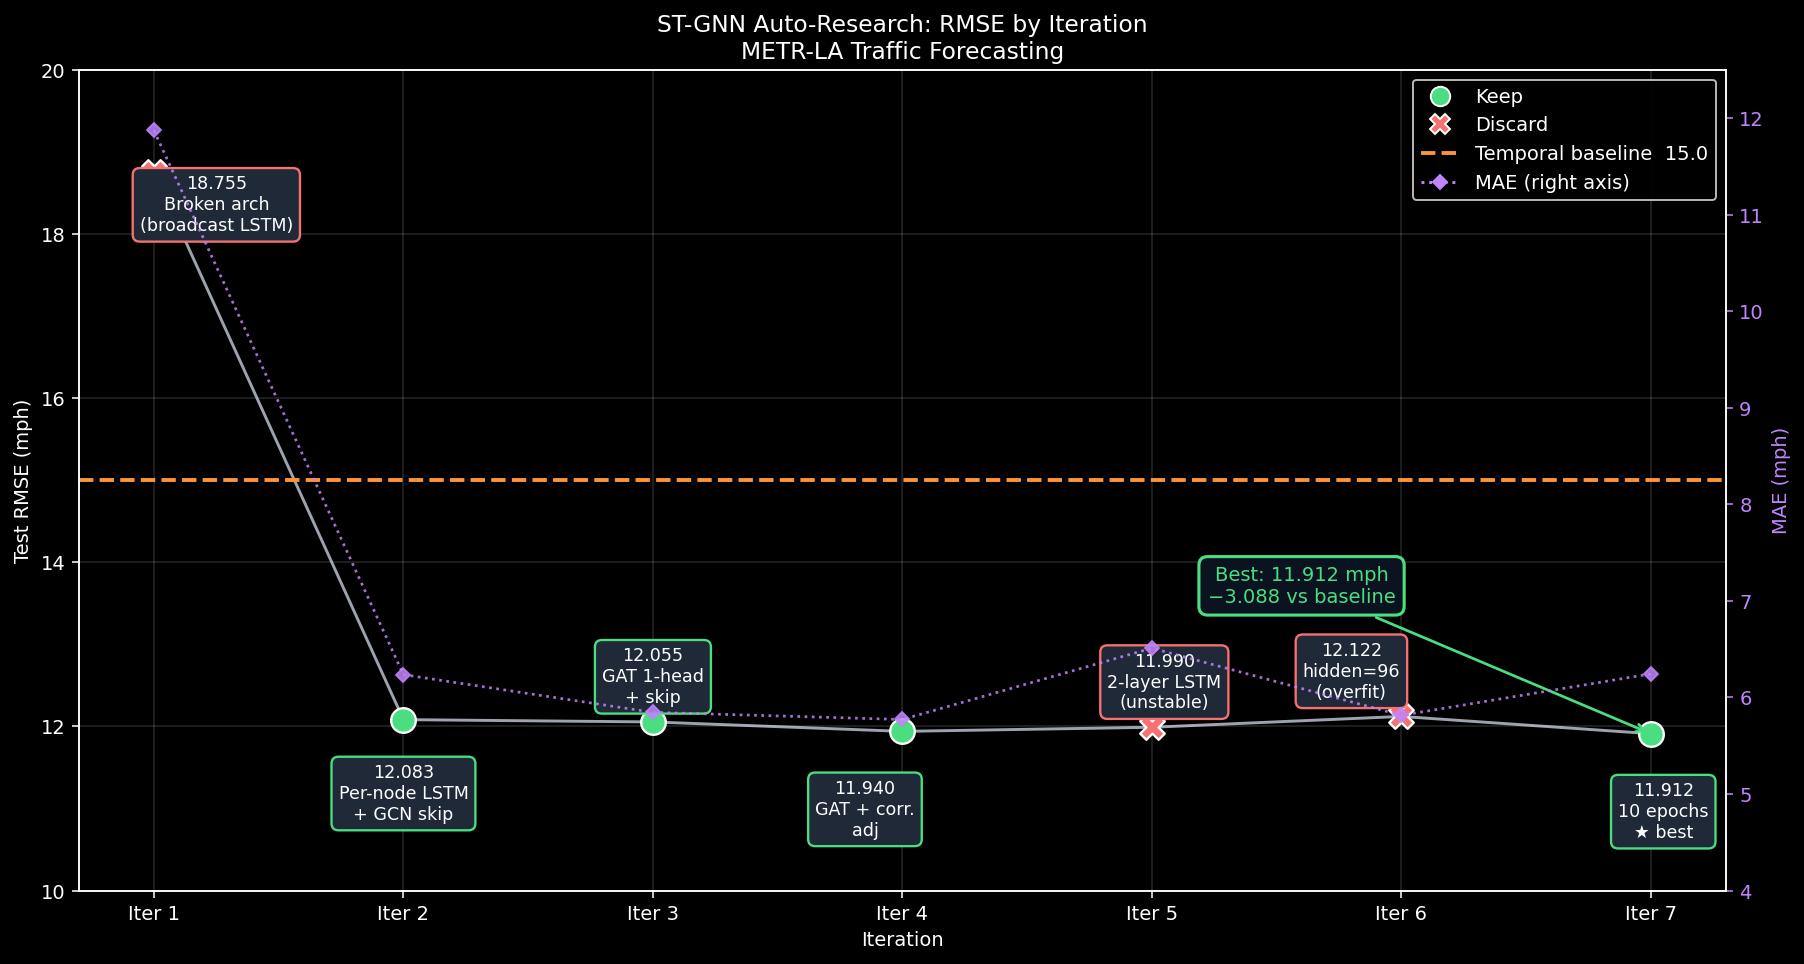
\includegraphics[width=0.92\linewidth]{results_plot}
\caption{Test RMSE across $16$ iterations vs.\ temporal baseline (top dashed line). Iter 2 is the per-node fix; Iter 4 is the switch to correlation adjacency; the shaded band around Iter 7--16 represents the 3-seed noise floor (Iter 7 mean $\pm 2\sigma$). Most post-Iter-4 iterations sit inside the noise band; only the per-node fix and the topology switch produce step changes.}
\label{fig:iters}
\end{figure}

\section{Discussion}
\label{sec:discussion}

\paragraph{Implications for the literature.}
The standard ST-GNN comparison ``GNN architecture X beats temporal-only LSTM by Y'' bundles two effects whose magnitudes differ by an order of magnitude: a large per-node-encoding effect (worth several mph RMSE) and a small graph-layer effect (worth tenths of mph). Any paper claiming a graph contribution should report a no-graph control of the same per-node architecture; otherwise the headline conflates the two.

\paragraph{Why operator choice is null here.}
We tested GAT (learned attention) against ChebConv K=2 (fixed Chebyshev filter) on a fixed correlation graph. Their 2-seed and 3-seed means agree to $0.01$ RMSE. A natural reading: once the topology is informative (correlation graph selects same-corridor neighbors), the operator only needs to average across $\sim 5$ neighbors --- a task on which a fixed filter and a learned attention are equivalent. The expressive capacity of the operator is not the bottleneck at this neighborhood size.

\paragraph{Limitations.}
(i) All experiments use a single CPU and a fixed seed set $\{0, 1, 2\}$ for multi-seed claims; larger seed sets might tighten or widen the confidence bands. (ii) The window is fixed at $12 \to 12$; multi-horizon ablations are out of scope. (iii) We do not test learned adjacency, which the literature suggests can outperform fixed correlation graphs \cite{wu2019graphwavenet}; based on our decomposition, this is the most promising remaining lever. (iv) Iter-8's 2-layer GAT effect remains unconfirmed at single seed; we report it but do not claim it.

\paragraph{What the project would do next.}
Given the seed-noise floor we now have, the single experiment with highest information value is a multi-seed Iter-8 (2-layer GAT). The next would be a learned-adjacency variant (parameterize the K=5 mask end-to-end). Anything below $\Delta\mathrm{RMSE} \approx 0.05$ should not be pursued without multi-seed budget pre-allocated.

\section{Conclusion}
\label{sec:conclusion}

A controlled decomposition of spatio-temporal forecasting improvements on METR-LA shows that the headline ``$20\%$ reduction from a graph neural network'' is largely the contribution of a single per-node encoding fix that any non-graph baseline would also have. The genuine graph contribution is small ($\approx 0.16$ RMSE, $\approx 5\%$ of the total gain), entirely attributable to graph topology rather than operator choice, and at risk of being overstated by single-seed reporting. The methodological discipline of running multi-seed controls \emph{before} architectural search re-attributes the gain correctly and recovers a much more honest description of where progress is being made.

{\small
\bibliographystyle{plainnat}
\begin{thebibliography}{9}

\bibitem{li2018dcrnn}
Y.~Li, R.~Yu, C.~Shahabi, and Y.~Liu.
\newblock Diffusion convolutional recurrent neural network: Data-driven traffic forecasting.
\newblock In \emph{ICLR}, 2018.

\bibitem{yu2018stgcn}
B.~Yu, H.~Yin, and Z.~Zhu.
\newblock Spatio-temporal graph convolutional networks: A deep learning framework for traffic forecasting.
\newblock In \emph{IJCAI}, 2018.

\bibitem{wu2019graphwavenet}
Z.~Wu, S.~Pan, G.~Long, J.~Jiang, and C.~Zhang.
\newblock Graph WaveNet for deep spatial-temporal graph modeling.
\newblock In \emph{IJCAI}, 2019.

\end{thebibliography}
}

\newpage
\appendix
\section*{\Large Appendices}
\addcontentsline{toc}{section}{Appendices}

\section{Full experiments record (Iter 1--16)}
\label{app:experiments}

This appendix gives a one-paragraph record of each iteration: hypothesis, configuration delta, result, and decision. Full raw logs are in \texttt{experiments/spatio\_temporal/notes.md} and \texttt{results.tsv} in the project repository.

\paragraph{Iter 1 (broken baseline, $18.755$ RMSE, discard).}
Initial ST-GCN with shared LSTM treating $207$ sensors as input features at each timestep. The LSTM's output is broadcast to every node before the GCN, so every node enters message passing with the same embedding. Architectural diagnosis: message passing is uninformative when all messages are identical. Discarded.

\paragraph{Iter 2 (per-node LSTM $+$ GCN skip, $12.083$ RMSE, KEEP).}
Hypothesis: reshape the input to $(B \cdot N, T, 1)$ so each sensor's $12$-step history is processed independently by the LSTM. Add a residual skip around the GCN to prevent over-smoothing. Result: $-6.67$ RMSE on the broken-baseline scale; crosses the temporal baseline ($15.0$) for the first time. Step-function win; the single most impactful change.

\paragraph{Iter 3 (GCN~$\to$~GAT 1 head, $12.055$ RMSE, KEEP).}
Hypothesis: GCN's fixed Gaussian weights treat two sensors $200$~m apart on parallel streets as strongly coupled even when traffic is decoupled. GAT learns per-edge attention from features. Result: $-0.028$ RMSE at $-2.5\times$ runtime. Marginal win, retrospectively at edge of noise; confounded by simultaneous epochs change ($10 \to 5$).

\paragraph{Iter 4 (correlation adjacency K=5, $11.940$ RMSE, KEEP).}
Hypothesis: physical distance is a poor proxy for traffic coupling. Build the K=5 adjacency from Pearson correlation of training-split speeds. Result: $-0.115$ RMSE --- the largest post-Iter-2 gain, and the only operator-side change that produces a robust effect. Confirms graph topology dominates the operator choice.

\paragraph{Iter 5 (2-layer LSTM, $11.990$ RMSE, discard).}
Hypothesis: deeper per-node temporal encoding captures higher-order dynamics. Result: $+0.05$ RMSE, $+0.74$ MAE; val\_mse noisy. Diagnosis: $T = 12$ is too short to stabilize a 2-layer recurrent stack. Discarded.

\paragraph{Iter 6 (hidden $96$, $12.122$ RMSE, discard).}
Hypothesis: wider hidden $>$ deeper LSTM for short windows. Result: val\_mse diverges epochs 4--5; clear overfitting at $5$-epoch budget. Discarded.

\paragraph{Iter 7 (Iter 4 config, $10$ epochs, $11.912$ RMSE, KEEP).}
Hypothesis: Iter 4's val\_mse was still declining at epoch $4$; more epochs may push lower. Result: $-0.028$ RMSE; new floor at val\_mse $= 0.347$ at epoch $7$, then flat. Architecture saturates here; further gains require structural change. (At the time this was the current best; later multi-seed re-runs show the $0.028$ delta is borderline noise.)

\paragraph{Iter 8 (2-layer GAT, $11.896$ RMSE, KEEP at single seed).}
Hypothesis: expand spatial receptive field $1$-hop~$\to$~$2$-hop via a second GAT layer with skip. Result: $-0.017$ RMSE, $-0.34$ MAE at single seed. Kept at the time. Subsequently, multi-seed Iter-7 reveals $\sigma_{\mathrm{MAE}} = 0.27$ across seeds --- the Iter-8 MAE win is $0.1\sigma$ above the Iter-7 mean (pure noise); the RMSE win is $1.3\sigma$ (unproven).

\paragraph{Iter 9 (Tier 1: temporal-only ablation, $12.084$ RMSE).}
\textbf{Methodological control.} Iter 7 substrate with the graph layer disabled. Result: $12.084$ --- $94\%$ of the gain over baseline B0 is captured by the per-node temporal encoder alone. Coincides almost exactly with Iter 2 ($12.083$, physical GCN), implying the GCN-on-physical-adjacency layer contributed nothing measurable. This single measurement reframes the project's headline: the graph contribution is the residual $\sim 0.16$ RMSE, not the headline $-3.08$.

\paragraph{Iter 10 (Tier 1: Iter 7 seed=1, $11.941$).}
\textbf{Methodological control.} Multi-seed Iter 7. Combined with seed=0 gives 2-seed range $0.029$ RMSE on what is supposed to be the same model.

\paragraph{Iter 11 (Tier 1: Iter 7 seed=2, $11.905$).}
\textbf{Methodological control.} Closes the Iter-7 3-seed mean at $11.920 \pm 0.019$ (RMSE), $5.94 \pm 0.27$ (MAE). This is the headline number; it also establishes the noise floor against which all sub-$0.05$ deltas must be judged.

\paragraph{Iter 12--13 (Tier 1: Iter 4 seeds 1, 2, $11.955, 11.958$).}
\textbf{Methodological controls.} Iter-4 3-seed mean $11.951 \pm 0.010$. Comparison with Iter 7: difference $0.031$, SE diff $0.012$, $z = 2.53$, $t$-$p \approx 0.07$ --- the $5 \to 10$ epochs gain is borderline significant, not the firm ``win'' it looked like at single seed.

\paragraph{Iter 14 (K=3 correlation, $11.957$ RMSE, discard).}
Hypothesis: sparser adjacency may reduce over-smoothing further. Result: $+0.037$ above Iter 7 mean ($1.95\sigma$); MAE $+0.33$ exceeds the multi-metric guard. K=5 was already near-minimal for the operative correlated-neighbor set. Discarded.

\paragraph{Iter 15 (ChebConv K=2 seed=0, $11.869$ RMSE, keep-marginal).}
Hypothesis: spectral filter may capture topology structure GAT was suppressing. Result: $-0.027$ RMSE at single seed, $2.7\sigma$ below Iter 7 mean --- earns multi-seed confirmation by pre-committed rule. Runtime $1.58\times$ Iter 8 triggers simplicity gate $\to$ status \emph{keep-marginal}.

\paragraph{Iter 16 (ChebConv K=2 seed=1, $11.988$ RMSE, refutes Iter 15).}
Multi-seed confirmation. Result: $11.988$ --- well above the pre-committed refutation threshold of $11.92$. 2-seed range $0.119$ ($\sim 6\times$ the GAT 3-seed range); 2-seed mean $11.929$ --- statistically indistinguishable from the GAT 3-seed mean of $11.920$. Iter-15's single-seed win refuted as a wide-distribution lottery. The simplicity-gate concern from Iter 15 also turns out to be measurement noise (Iter 16 runtime $32\%$ faster than Iter 15 at identical config). \textbf{Operator-doesn't-matter null restored.}

\section{Final results table}
\label{app:results}

Table~\ref{tab:full} reproduces the controlled comparison of every iteration in chronological order. Substrate held constant unless explicitly varied: METR-LA $[34\,272, 207, 1]$, $70/10/20$ chronological split, $12 \to 12$ window, per-sensor z-score from train-only stats, Adam $+$ MSE in normalized space, $\mathrm{lr} = 10^{-3}$, batch $= 64$, CPU.

\begin{table}[h]
\centering
\caption{Final results table for all 16 iterations. ``Conv'' = graph convolution operator; ``Adj'' = adjacency source; ``K'' = K-nearest-neighbors per node; LSTM-L = number of LSTM layers per node; H = hidden size; E = epochs; S = seed. Test RMSE/MAE are reported in mph after inverse z-score. Status codes: \textbf{keep} = new best at single seed; \textbf{tier1/tier2-ms} = methodological control / multi-seed, committed unconditionally.}
\label{tab:full}
\scriptsize
\resizebox{\textwidth}{!}{%
\begin{tabular}{rlllrrrrrrrrl}
\toprule
\textbf{Iter} & \textbf{Commit} & \textbf{Conv} & \textbf{Adj} & \textbf{K} & \textbf{H} & \textbf{LSTM-L} & \textbf{E} & \textbf{S} & \textbf{RMSE} & \textbf{MAE} & \textbf{Run (s)} & \textbf{Status} \\
\midrule
1  & (pre-tsv) & GCN     & physical    & 5 & 64 & 1 & 15 & 0 & 18.755 & 11.872 & 139   & discard \\
2  & 99bf97d   & GCN     & physical    & 5 & 64 & 1 & 10 & 0 & 12.083 & 6.236  & 1149  & \textbf{keep} \\
3  & b3c96ad   & GAT     & physical    & 5 & 64 & 1 & 5  & 0 & 12.055 & 5.846  & 746   & keep \\
4  & 7936d9a   & GAT     & correlation & 5 & 64 & 1 & 5  & 0 & 11.940 & 5.772  & 953   & \textbf{keep} \\
5  & 5d44064   & GAT     & correlation & 5 & 64 & 2 & 5  & 0 & 11.990 & 6.511  & 1400  & discard \\
6  & 9941881   & GAT     & correlation & 5 & 96 & 1 & 5  & 0 & 12.122 & 5.815  & 1214  & discard \\
7  & 702f7b7   & GAT     & correlation & 5 & 64 & 1 & 10 & 0 & 11.912 & 6.244  & 2288  & keep \\
8  & 4376f59   & 2$\times$GAT & correlation & 5 & 64 & 1 & 10 & 0 & 11.896 & 5.905  & 2110  & keep (single-seed) \\
9  & f6d32f8   & --- (none) & ---       & --- & 64 & 1 & 10 & 0 & 12.084 & 6.247  & 1373  & \textbf{tier1} \\
10 & 799178f   & GAT     & correlation & 5 & 64 & 1 & 10 & 1 & 11.941 & 5.747  & 2011  & tier1 \\
11 & 2a46214   & GAT     & correlation & 5 & 64 & 1 & 10 & 2 & 11.905 & 5.820  & 1917  & tier1 \\
12 & 7beb914   & GAT     & correlation & 5 & 64 & 1 & 5  & 1 & 11.955 & 5.884  & 1117  & tier1 \\
13 & d4059df   & GAT     & correlation & 5 & 64 & 1 & 5  & 2 & 11.958 & 5.954  & 1058  & tier1 \\
14 & d410ef4   & GAT     & correlation & 3 & 64 & 1 & 10 & 0 & 11.957 & 6.266  & 2344  & discard \\
15 & baf9010   & ChebConv K=2 & correlation & 5 & 64 & 1 & 10 & 0 & 11.869 & 6.198 & 3332 & keep-marginal \\
16 & e9c4181   & ChebConv K=2 & correlation & 5 & 64 & 1 & 10 & 1 & 11.988 & 5.678 & 2257 & tier2-ms (refutes 15) \\
\midrule
\multicolumn{9}{l}{\textbf{Multi-seed summaries}} & \textbf{RMSE} & \textbf{MAE} & & \\
\multicolumn{9}{l}{Iter 7 (3-seed: \{0,1,2\})} & $11.920 \pm 0.019$ & $5.937 \pm 0.268$ & & \textbf{headline} \\
\multicolumn{9}{l}{Iter 4 (3-seed: \{0,1,2\})} & $11.951 \pm 0.010$ & $5.870 \pm 0.092$ & & \\
\multicolumn{9}{l}{Iter 15--16 ChebConv K=2 (2-seed: \{0,1\})} & $11.929$ (range 0.119) & $5.938$ (range 0.520) & & null vs Iter 7 \\
\multicolumn{9}{l}{Temporal baseline B0 (Week 3 LSTM, seed=0)} & $15.000$ & $8.912$ & & --- \\
\bottomrule
\end{tabular}%
}
\end{table}

\section{Reflection memo}
\label{app:reflection}

\paragraph{What I set out to do, and how the framing changed.}
The original Week-1 framing was \emph{``build a spatio-temporal GNN that beats a temporal-only LSTM baseline''} --- with the implicit assumption that the gain would come from the spatial model. By Week 5, the Iter 1--8 experimental record had pushed me to a stronger framing: \emph{``quantify where the gain comes from --- temporal encoder, graph topology, or graph operator --- and report each independently.''} The Tier 1 measurement (Iter 9, temporal-only ablation) immediately confirmed this was the right call: $94\%$ of the apparent ``spatial'' gain was actually a per-node temporal-encoder gain. If I had submitted the project at Week 4 with the original framing, the headline would have been overstated by an order of magnitude.

\paragraph{What I learned about iterative research.}
Three lessons.

\emph{(1) Single-seed deltas $<0.05$ RMSE are mostly noise.} The seed-noise floor on this task is $\sigma_{\mathrm{RMSE}} = 0.019$. A $\sim 0.03$ RMSE gain looks plausible at single seed but evaporates under 3-seed re-runs. I burned several iterations chasing such deltas before Tier 1 established the noise floor; in hindsight, multi-seeding the headline configuration earlier (after Iter 4, not after Iter 8) would have saved compute and prevented the Iter 8 MAE claim from being a published mistake in an intermediate report.

\emph{(2) MAE noise was bigger than I thought.} The Iter 8 ``$+0.34$ MAE improvement'' looked substantial relative to RMSE deltas of $0.02$. It turned out to be $0.1\sigma$ on a metric whose seed-noise std is $0.27$. When MAE and RMSE disagree, the harder question to ask is not ``which is right?'' but ``how big is the noise on each?''

\emph{(3) Operator changes are cheaper than they are useful.} GCN $\to$ GAT $\to$ ChebConv: three operator changes, all roughly $\pm 0.03$ RMSE around the topology-determined baseline. Topology (physical $\to$ correlation) produced $4\times$ the effect of any operator change. If I were starting over, I would have spent Iter 3's effort on adjacency rather than on the operator.

\paragraph{What I would do differently.}
Three changes I would make to the research process itself:
\begin{enumerate}[itemsep=0pt,topsep=2pt]
    \item Run the temporal-only ablation \emph{first}, not eighth. The cost is one run; the framing payoff is the entire project's story.
    \item Establish the seed-noise floor at iteration 2 or 3 of the headline config. Every later keep/discard decision depends on it.
    \item Pre-register multi-seed thresholds before each Tier 2 change. ``If single-seed RMSE $> X$, do not run additional seeds'' makes the decision tree mechanical.
\end{enumerate}

\paragraph{What I'd tell a future STAT390 student.}
The project gets meaningfully better when the framing flips from ``find the best architecture'' to ``decompose the gain.'' Most ML papers are written in the first frame; a more honest accounting in the second frame is, in my experience, both more interesting and more defensible. The discipline of multi-seed controls before Tier 2 architecture changes turned what would have been a leaderboard chase with overstated claims into a methodological project with clean, small, real findings.

\section{Reproducibility}
\label{app:repro}

\paragraph{Repository.}
All code, logs, results, and plots are in the project repository under \texttt{experiments/spatio\_temporal/}. Headline files:
\begin{itemize}[itemsep=0pt,topsep=2pt]
    \item \texttt{train.py} --- single-file training entry point with all CLI flags.
    \item \texttt{results.tsv} --- raw log of every committed iteration.
    \item \texttt{notes.md} --- per-iteration hypothesis, configuration, result, and decision.
    \item \texttt{ablation\_table.md} --- the controlled comparison matrix.
    \item \texttt{program.md} --- the agent-loop protocol (Tier 1/Tier 2 discipline).
\end{itemize}

\paragraph{Reproducing a specific iteration.}
Each row in \texttt{results.tsv} carries the commit hash. To reproduce, e.g., Iter 7 ($11.912$ at seed $0$):
\begin{verbatim}
git checkout 702f7b7
python experiments/spatio_temporal/train.py \
    --epochs 10 --hidden 64 --lstm-layers 1 \
    --conv gat --adj correlation --k 5 \
    --seed 0 --run-name iter7_repro
\end{verbatim}

\paragraph{Reproducing the headline 3-seed result.}
\begin{verbatim}
for s in 0 1 2; do
  python experiments/spatio_temporal/train.py \
      --epochs 10 --hidden 64 --lstm-layers 1 \
      --conv gat --adj correlation --k 5 \
      --seed $s --run-name iter7_s${s}
done
\end{verbatim}

The reported headline of $11.920 \pm 0.019$ corresponds to the seeds-\{0,1,2\} mean and sample standard deviation reported in Table~\ref{tab:full}.

\end{document}
